\chapter{End Effector Design}
\label{sec:ee_design}

The design of the end effector (EE) required navigating an expansive design space, as picking solutions are heavily dependent on the mechanical properties of the target objects. Our system is designed for high generality; it must package and palletize not only microwaves but also non-uniform surfaces and thermocouples. Three primary architectural approaches were evaluated:

\begin{itemize}
    \item \textbf{Purely Mechanical:} Utilizing side-gripping or form-closure fingers.
    \item \textbf{Purely Vacuum:} Utilizing suction cup arrays and continuous evacuation.
    \item \textbf{Hybrid:} A combination of mechanical support and vacuum adhesion.
\end{itemize}

While a hybrid approach is often theorized as a balanced solution, a purely vacuum system was determined to be optimal for this application. This selection was based on simplicity of design, which inherently increases system reliability and generality. Experimental validation confirmed that the vacuum system is viable even when gripping through protective plastic films, as the evacuation process utilizes external atmospheric pressure to rigidly "clamp" the suction cup interface to the microwave chassis.

\section{Design Selection and Material Analysis}

\subsection{Mechanical Constraints}
Initial designs focused on mechanical side-gripping. However, the force requirements exceeded the material limits of the packaging. Dawlance utilizes 5-layer B+B corrugated cardboard (3mm flute size). To hold a 40kg microwave via friction alone, the required normal force $F_n$ is calculated using an estimated coefficient of friction $\mu = 0.4$:

$$ F_f = \mu \cdot F_n \implies (40\text{kg} \times 10\text{N/kg}) = 0.4 \cdot F_n \implies F_n = 1000\text{N} $$

Structural analysis (including edge, box, and face crushing tests) indicated that the cardboard joints fail at approximately 200N. Thus, a force-closure mechanical grip would cause material failure before achieving the necessary frictional hold.

\subsection{Vacuum Feasibility}
The vacuum system was tested with thermocouples and microwaves through plastic. Prototypes successfully lifted up to 40kg (verified with calibrated weights). To mitigate horizontal slippage during high-speed movement, path optimization was performed using a trapezoidal trajectory profile. With a 10s cycle time, the maximum acceleration is limited to $0.5\text{m/s}^2$. For a 40kg payload, this results in a horizontal shear force of:

$$ F_{shear} = m \cdot a = 40\text{kg} \times 0.5\text{m/s}^2 = 20\text{N} $$

By balancing the center of mass between the suction cups, this force is distributed to 10N per primary contact point, which falls within the safe operating envelope of the selected grippers.

\section{Suction Cup Array and Vacuum System}

\subsection{Array Configuration}
The redesigned array consists of two large center suction cups (125mm bellows) and four peripheral smaller cups (50mm). Bellows-type cups were selected for their superior compliance on non-uniform surfaces, despite their larger internal volume.

\subsection{Vacuum Calculations}
The system is constrained by a target gripping engagement time of 200ms to 400ms. 

\textbf{Total System Volume Calculation:}
\begin{itemize}
    \item \textbf{Suction Cups:} 2 x 125mm cups at $307\text{cm}^3$ each = $614\text{cm}^3$.
    \item \textbf{Piping:} 8mm diameter tubing, 3m length:
    $$ V_{pipe} = \pi \cdot r^2 \cdot L = \pi \cdot (0.4\text{cm})^2 \cdot 300\text{cm} \approx 150.8\text{cm}^3 $$
    \item \textbf{Total Volume ($V_{total}$):} $\approx 764.8\text{cm}^3$ (0.765 Liters).
\end{itemize}

\textbf{Evacuation Performance:}
To achieve a 0.5 bar absolute vacuum within 400ms, the required flow rate $Q$ is estimated:
$$ Q = \frac{V_{total} \cdot \ln(P_{atm}/P_{final})}{t} = \frac{0.765 \cdot \ln(1/0.5)}{0.4/60} \approx 79.5\text{L/min} $$
With the 5bar compressor provided by Dawlance and our current vacuum pump rated at 92.6L/min, the system theoretically meets the 400ms requirement, assuming leakage is minimized via the implemented Teflon sealing and top-oriented bolt configurations.

\section{Yaw Axis and Structural Framework}

\subsection{Yaw Axis Design}
The yaw axis utilizes a shaft supported by two angular contact ball bearings in a face-to-face (DF) configuration. This setup was chosen over back-to-back (DB) for ease of mounting on the 2mm main plate. FEA simulation in Fusion360 confirmed that this configuration safely handles the 40kg static load. Earlier iterations using stepped shafts or separate radial/thrust bearings were abandoned due to manufacturing complexity and assembly constraints within the 4-5mm wall thickness of the hollow sections.

\subsection{Structural Support}
The frame consists of aluminum 40/40 extrusions in a quadrilateral arrangement. The suction cup array is mounted to a main board via a sandwiched plate, with T-nuts used for securing the custom brackets to the extrusions.

\begin{figure}[H]
    \centering
    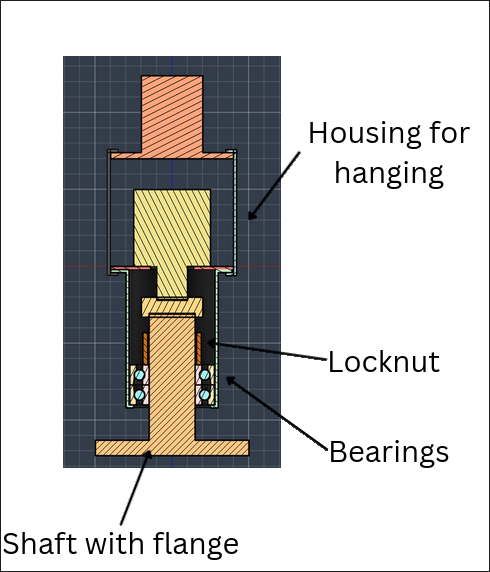
\includegraphics[width=1\linewidth]{EE_CAD.png}
    \caption{End Effector CAD assembly highlighting the yaw axis and suction array.}
    \label{fig:ee_cad}
\end{figure}

\begin{figure}[H]
    \centering
    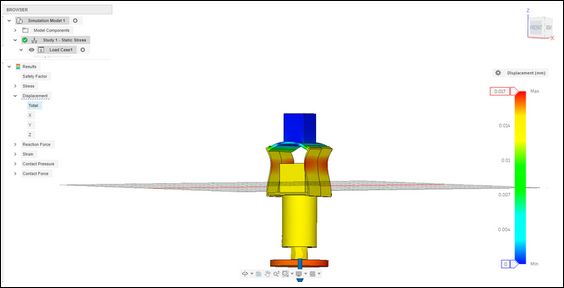
\includegraphics[width=0.8\linewidth]{EE_Simulation.png}
    \caption{FEA results showing stress distribution under a 40kg load.}
    \label{fig:ee_simulation}
\end{figure}

\section{Summary of Results}
The final design utilizes six suction cups (SMC 80mm equivalents or Festo 125/50mm mix). At 40kPa of vacuum, the theoretical lift capacity is 123kg. Accounting for a 65\% efficiency factor for semi-porous surfaces, the system provides a safe lift of ~80kg, yielding a safety factor of 2 for the heaviest expected payload.